\documentclass[twocolumn,a4j]{jsarticle}
\setlength{\topmargin}{-20.4cm}
\setlength{\oddsidemargin}{-10.4mm}
\setlength{\evensidemargin}{-10.4mm}
\setlength{\textwidth}{18cm}
\setlength{\textheight}{26cm}

\usepackage[top=15truemm,bottom=20truemm,left=20truemm,right=20truemm]{geometry}
\usepackage[latin1]{inputenc}
\usepackage{amsmath}
\usepackage{amsfonts}
\usepackage{amssymb}
\usepackage[dvipdfmx]{graphicx}
\usepackage[hang,small,bf]{caption}
\usepackage[subrefformat=parens]{subcaption}
\usepackage[dvipdfmx]{color}
\usepackage{listings}
\usepackage{listings,jvlisting}
\usepackage{geometry}
\usepackage{framed}
\usepackage{color}
\usepackage[dvipdfmx]{hyperref}
\usepackage{ascmac}
\usepackage{enumerate}
\usepackage{tabularx}
\usepackage{cancel}
\usepackage{scalefnt}
\usepackage{overcite}
\usepackage{otf}
\usepackage{multicol}
\usepackage[geometry]{ifsym}

\renewcommand{\figurename}{Fig.}
\renewcommand{\tablename}{Table }

\hypersetup{%
    hidelinks %リンクの色消し
}

\lstset{
basicstyle={\ttfamily},
identifierstyle={\small},
commentstyle={\smallitshape},
keywordstyle={\small\bfseries},
ndkeywordstyle={\small},
stringstyle={\small\ttfamily},
frame={tb},
breaklines=true,
columns=[l]{fullflexible},
xrightmargin=0zw,
xleftmargin=3zw,
numberstyle={\scriptsize},
stepnumber=1,
numbersep=1zw,
lineskip=-0.5ex
}

% キャプション後ろのダブルコロンを消す
\makeatletter
\long\def\@makecaption#1#2{%
  \vskip\abovecaptionskip
  \iftdir\sbox\@tempboxa{#1\hskip1zw#2}%
    \else\sbox\@tempboxa{#1 #2}%
  \fi
  \ifdim \wd\@tempboxa >\hsize
    \iftdir #1\hskip1zw#2\relax\par
      \else #1 #2\relax\par\fi
  \else
    \global \@minipagefalse
    \hbox to\hsize{\hfil\box\@tempboxa\hfil}%
  \fi
  \vskip\belowcaptionskip}
\makeatother


\makeatletter
\def\@maketitle
{
\begin{center}
{\LARGE \@title \par}
\end{center}
\begin{flushright}
{\large \@date}\\
{\large 京都工芸繊維大学 大学院 機械設計学専攻 計測システム工学研究室}\\
{\large M2 \@author}
\end{flushright}
\par\vskip 1.5em
}
\makeatother

\author{来代 勝胤 / KITADAI Masatsugu}
\title{令和5年度 9月度 月例報告書}
\date{2023/09/20}

\begin{document}
\columnseprule=0.1mm
\maketitle

\section*{報告内容}
\begin{enumerate}[1.]
	\item ISTP-33 の内容について
	\item 粒子像の取得アルゴリズムの改善
	\item 10月の予定
\end{enumerate}

\section*{進捗報告}
8,9月は ISTP の発表に向けた資料の作成および
粒子像の取得アルゴリズムの改善を行った.

\section{ISTP-33 の内容について}
\begin{table}[hbtp]
	\label{table:data_type}
	\begin{tabular*}{80mm}{ c | c }
		\hline
		\textgt{題目} & \begin{tabular}{c} Performance Evaluation of \\ PIV Measurement of Secondary Flow \\ using Multi-Color LLS \end{tabular}        \\ \hline
		\textgt{内容} & \begin{tabular}{c} 数値シミュレーションを用いた\\計測手法の精度評価の結果について \end{tabular}        \\ \hline
		\textgt{日時} & 2023/9/24 - 9/27                 \\ \hline
		\textgt{会場} & 熊本県 熊本市中央区 熊本城ホール\\ \hline
	\end{tabular*}
\end{table}

\subsection{Contents}
\begin{enumerate}[(1)]
	\item Background and Motivations
	\item Objectives
	\item Mesurement Method
	\item Numerical Simulation
	\item Results
	\item Conclusions
\end{enumerate}
※ 詳細は資料 2ページ以降参照

\section{粒子像の取得アルゴリズムの改善}
\subsection{粒子特定の手順}
\begin{itemize}
	\item 撮影画像の平均値を用いた背景処理
	\item 混色の割合の計算し,カラーフィルタを作成
	\item カラーフィルタを用いた粒子像の識別 (B or G)
	\item 平均フィルタによる輝度分布の平滑化
	\item マスク画像を用いて粒子位置を特定
\end{itemize}

\newpage
\begin{figure}[htbp]
	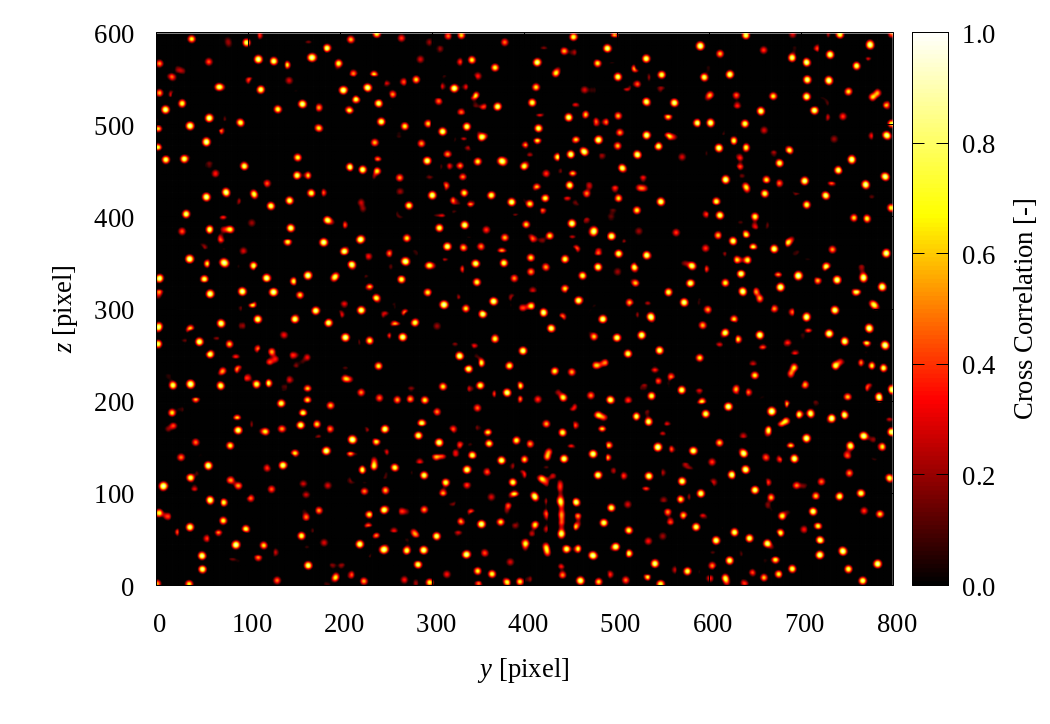
\includegraphics[keepaspectratio, width=82mm]{../images/cross_crr_particle.png}
	\caption{Cross correlation of particles image : Green}
	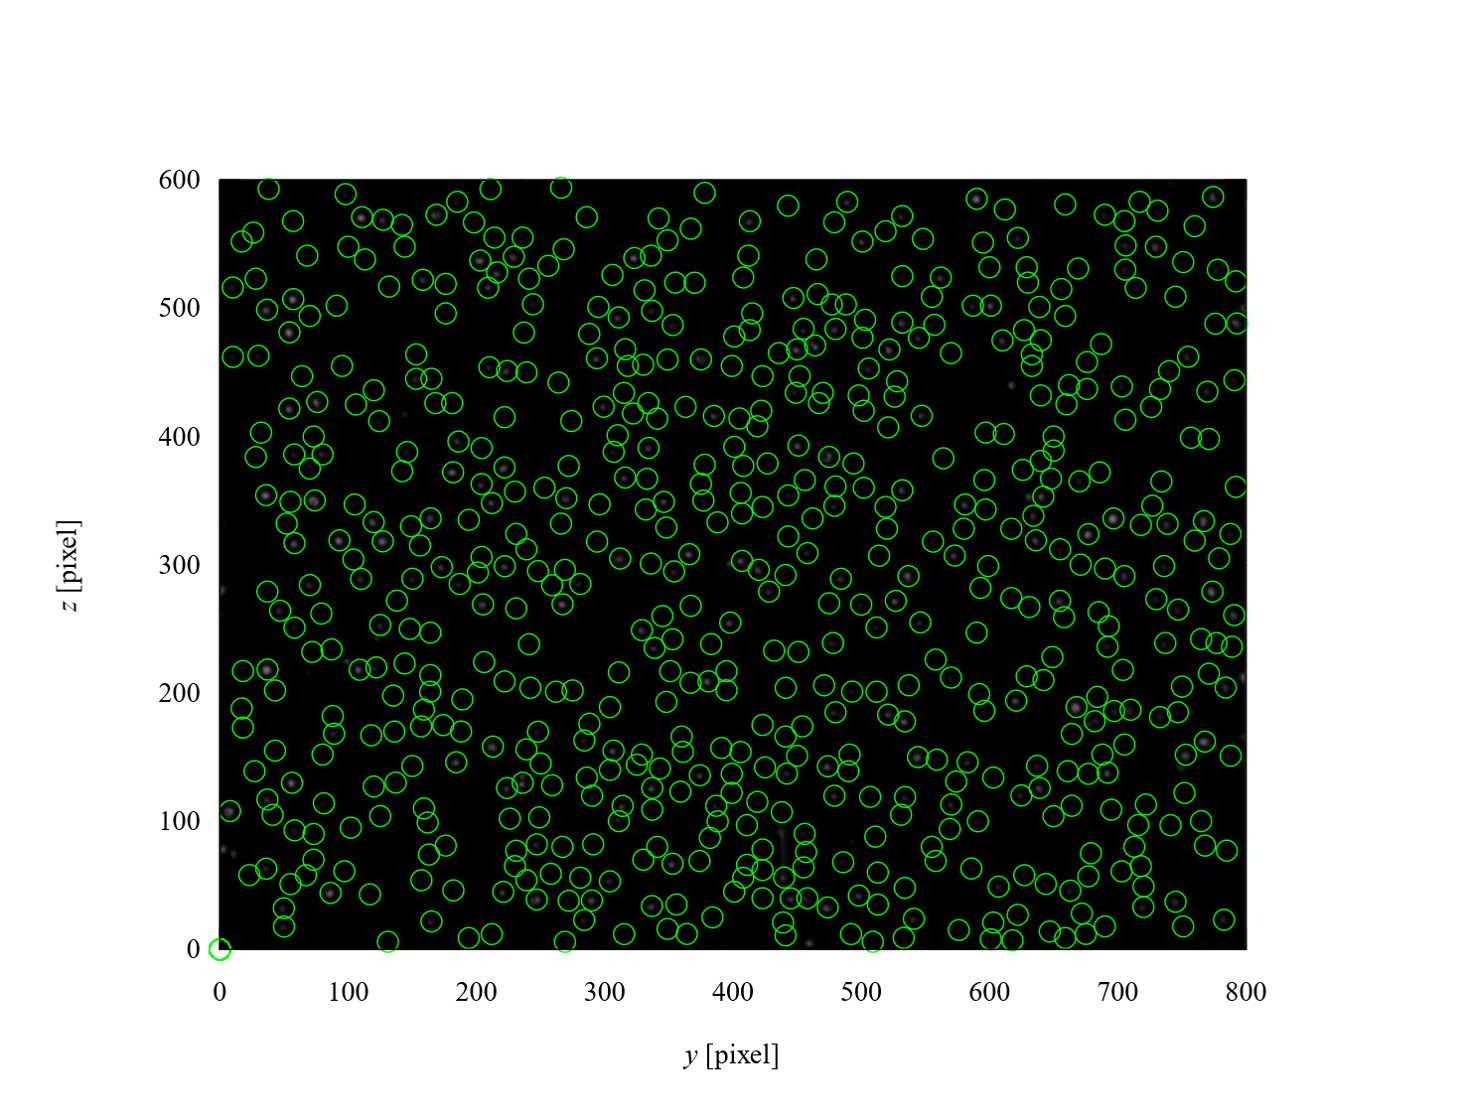
\includegraphics[keepaspectratio, width=82mm]{../images/particle_positions_green.png}
	\caption{Particles positions : Green}
\end{figure}

\begin{table}[hbtp]
	\centering
	\caption{Particle detection for green image}
	\begin{tabular}{l c}
		\hline
		Method of particle detection & Number of particles \\ \hline \hline
		Binarization images          & 100                 \\ \hline
		Cross correlation plane      & 200                 \\ \hline
	\end{tabular}
\end{table}

\section{10月予定}
\begin{itemize}
	\item ISTP-33 (9/24-27)
	\item 解析アルゴリズムの改善
\end{itemize}

\end{document}